%!TEX root = main.tex
\section{Recurrent Neural Network: Prediction} \label{sec:rnn_pred}

In addition to classification, we also investigated applying LSTMs to the task of pedestrian motion prediction.
That is, rather than a binary label, we try to predict \textit{where} the pedestrian will walk next.
This is much more challenging, but also would be more insightful to an end-user in vehicle applications.

\subsection{Introduction}
Existing research has been conducted in predicting trajectories in a 2D space. 
One relevant work used LSTMs to generate human handwriting from the IAM online handwriting database~\cite{DBLP:journals/corr/Graves13}~\cite{otoro}.

LSTMs can be used to predict sequences, by feeding themselves their output as an input.
To switch from binary classification to trajectory predicting LSTM, we change the network architecture from many-to-one to many-to-many.
The output $y_t \in \Re^{T\text{x}2}$ is computed from every time step as given in ~\cref{eq:bin_class_out}.

Many works can be found for the task of text prediction (e.g. \cite{ICML2011Sutskever_524}).
However, our application domain is real-valued, as opposed to the discrete-valued domain of word prediction.

The literature proposes several transformations, which could be applied to the output $y_t$.
For example, \cite{DBLP:journals/corr/Graves13} uses mixture density networks (MDNs) to calculate $x_{t+1}$ with the conditional probability $P(x_{t+1}|y_t)$, with parameters of the distribution: mean $\mu_m$, standard deviation $\sigma_m$, correlation $\rho_m$, mixture weights $\pi_m$ for $M$ mixture components.

Additionally, \cite{DBLP:journals/corr/Graves13} used the relative position between timesteps $\delta x = x_{t+1} - x_t$ as input vector.
In our case, we cannot use the relative position, because we would lose the information of proximity to the car.
In other words, we would ignore that a pedestrian might avoid an approaching car.
For the MDN approach, our means $\mu_m$ would be further spread among the full absolute position space, which would presumably require even longer training time than the earlier approach.
Therefore, we have decided to linearly compute the output, as stated in ~\cref{eq:bin_class_out}. 

Our chosen loss function is the mean squared error of each predicted output and next ground truth input, over the whole time sequence.
We have used the $L_2$ norm instead of the $L_1$ norm to be more robust against outliers.

\begin{equation}
Loss_{pred}(x_t) = \frac{1}{T} \sum_{t=0}^{T}(y_t - x_{t+1})^2
\label{eq:loss_pred} 
\end{equation}
%TODO write about last point.

% random batch
The loss function is computed for every batch and we update the parameters in the activation cells via AdamOptimizer.
We randomly draw batches from our training dataset for each parameter update to break dependencies of neighboring trajectory snippets in the training set.

% prediction, parameter-sharing
For prediction, the parameter-sharing property of RNNs and LSTMs is essential.
The activation units' parameters have been trained to predict the next state based on the current state.
Therefore, for prediction, where the ground truth input vector is unkown, the LSTM can use the output $y_{t-1}$ as input for $x_t$.
This gives us the predicted pedestrian position $y_t$.

\subsection{Generated Data}
As seen in the previous sections, pedestrian trajectories are highly complex nonlinear functions.
To validate our LSTM prediction model, we have instead tested on simpler functions; we generated linear and sinusoidal shaped trajectories, displayed in ~\cref{fig:lin_sin_traj}.

\begin{figure}
	\centering
	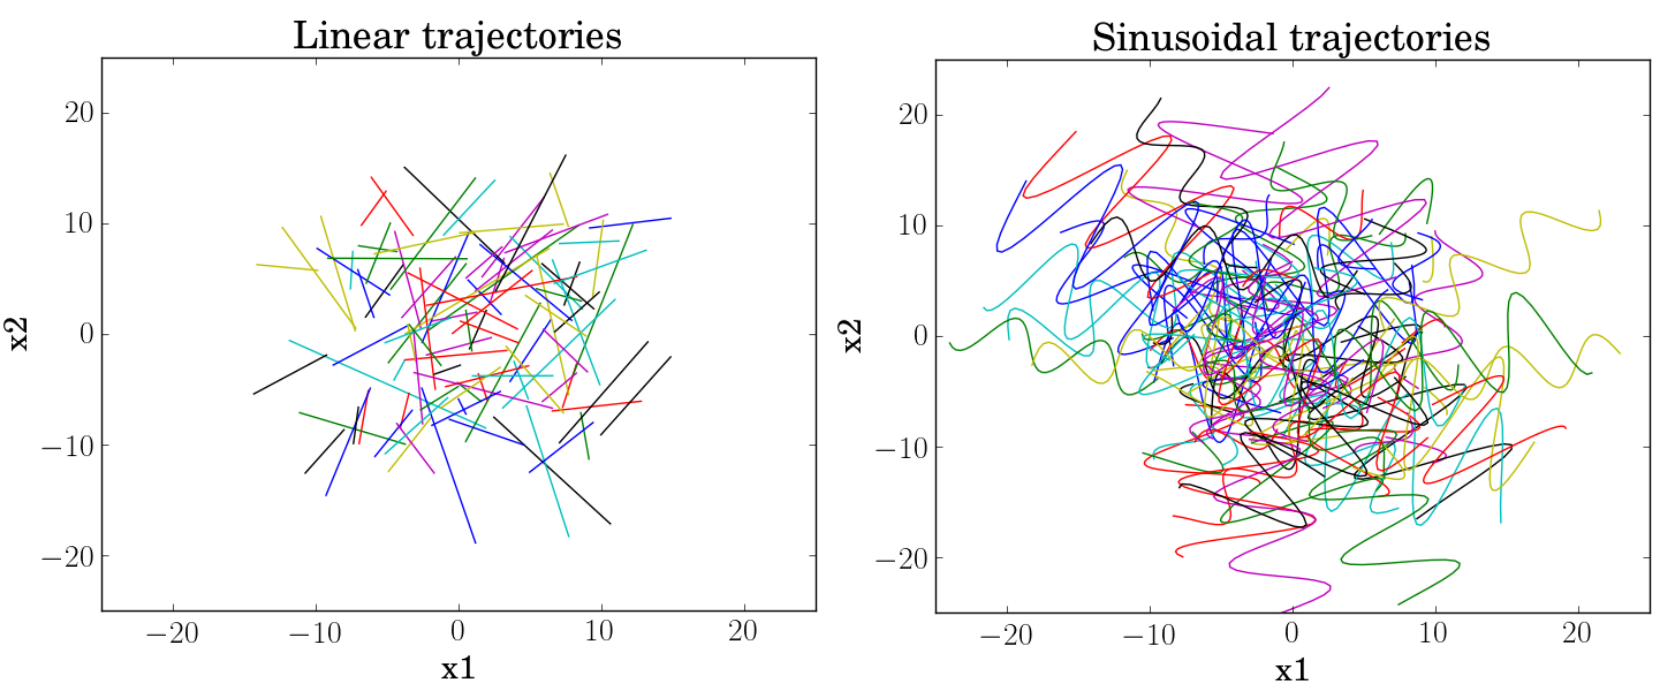
\includegraphics [trim=0 0 0 0, clip, angle=0, width=1.0\columnwidth,
	keepaspectratio]{figures/lin_sin_traj}
	\caption{Randomly generated trajectory data in linear (left) shape and sinusoidal shape (right). The trajectories have been generated by sampling the start point, range, scale, translation and rotation at random.} 
	\label{fig:lin_sin_traj} 
\end{figure}
%TODO fit linear data
For our hyperparameter tuning, we considered the batch size $b$, number of training samples $N$, snippet length $T$, learning rate $lr$, maximum epochs $e_{max}$ and number of hidden units $n_h$. 
As the possible combinations rise exponentially with the number of parameters and our computational resources are finite, we have evaluated most of the parameters, while holding the other parameters constant.
Optimal tuning would run a search over all combinations, which would result in better performance.

As seen in ~\cref{fig:rnn_hidden}, the number of hidden units $n_h = 1$ is insufficient to represent the complexity of sinusoidal curves.
We can also see that the complexity of $n_h=4$ is sufficient to approximately fit the sinusoidal shape, and $n_h=32$ is sufficient to fit the data accurately upon visual inspection.


\begin{figure}
	\centering
	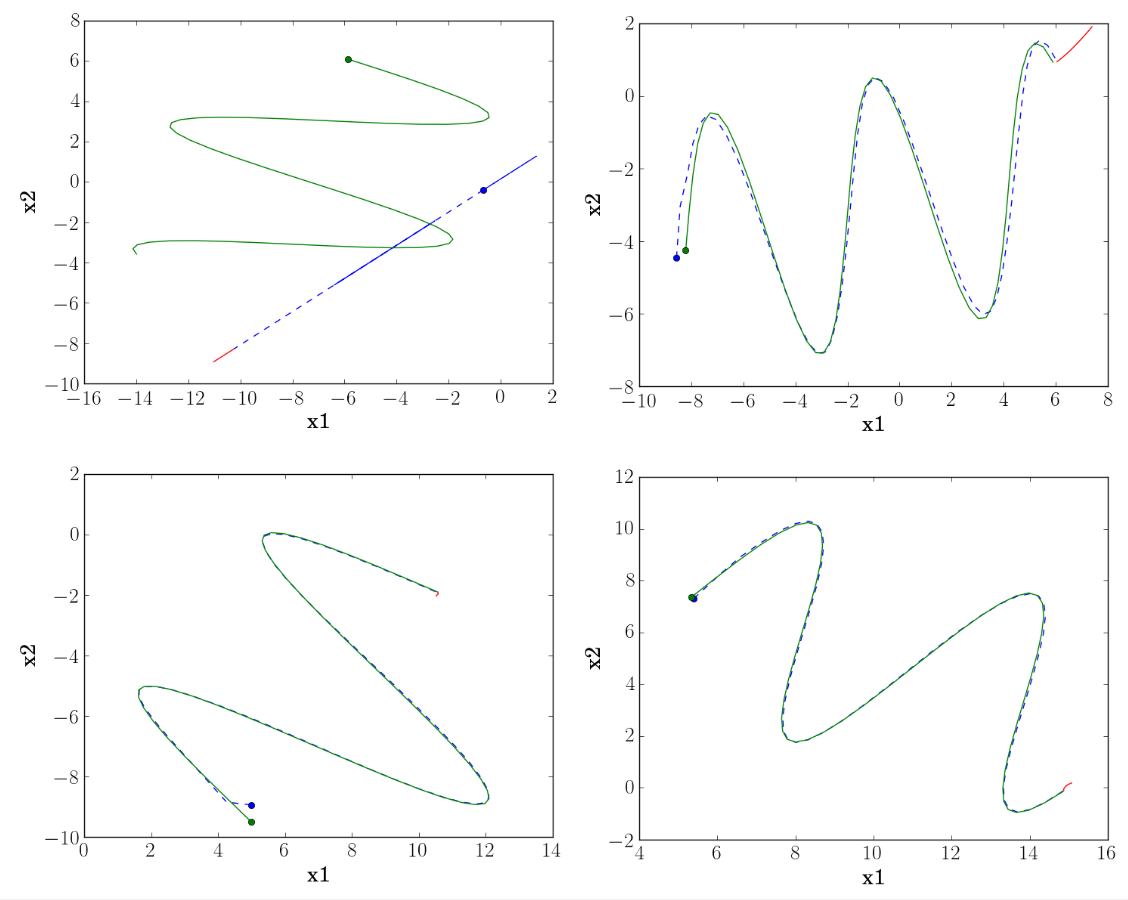
\includegraphics [trim=0 0 0 0, clip, angle=0, width=1.0\columnwidth,
	keepaspectratio]{figures/rnn_hidden}
	\caption{Search over the number of hidden units: $n_h=1$(top-left), $n_h=4$(top-right), $n_h=32$(bottom-left), $n_h=128$(bottom-right). The plot displays the input trajectory (green) $x_t$ with total trajectory snippet length $T=50$ an its starting point (green-dot). The LSTM predicts the next pedestrian position $y_t$ (blue-dotted) with its starting point (blue-dot), based on the past sequence $x_{0:t}$ and the learned parameters. After the input trajectory (green) is finished, the LSTM tries to predict the future trajectory (red) for $T_p=10$ timesteps. All trajectories are test trajectories and have not been included in the training set. LSTM was also able to predict for linear trajectories -- we have chosen to show the more interesting sinusoidal curves. The first blue dot $y_0$ purely based on the input $x_0$, and therefore deviates from the green curve.}
	\label{fig:rnn_hidden}
\end{figure}

In ~\cref{tab:rnn_hidden} we see that the loss shrinks with an increasing number of hidden nodes $n_h$.
The training time dramatically increases with the number of hidden units.
A high number of hidden units corresponds to high model complexity (and high bias), which could lead to overfitting on the training data.
However, we do not observe symptoms of overfitting, as accuracy is similar on training and test data.
The more complex the model, the fewer epochs it took to reach an acceptable loss value.
Moving forward, we refer to the models with the hyperparameters from ~\cref{tab:rnn_hidden} as 1-, 4-, 32- and 128-unit model.

We used early stopping (based on a validation dataset) to prevent overfitting.
The training was stopped when the difference in average batch loss between two consecutive epochs $\delta L_b < 0.001$.


\begin{table}[]
\centering
\begin{tabular}{ c| c| c| c| c}
& $n_h=1$ & $n_h=4$ &$n_h=32$ & $n_h=128$\\
\hline
$L_e=0$ & 58.5 & 49.7  & \textbf{6.22} & 2.62      \\
$L_e=1$ & 54.2 & 36.0  & \textbf{0.50} & 0.12      \\
$L_e=2$ & 51.1 & 24.4  & \textbf{0.23} & 0.05      \\
$L_e=3$ & 49.2 & 17.8  & \textbf{0.14} & 0.03      \\
\hline
$e_c$ 			& 25 	& 85 	& 35	& 10 		\\
$L_{e_c}$		&  0.30	& 0.03	& 0.0058& 0.004 	\\
$L_{test, e_c}$	& 0.34	& 0.04	&0.003	& 0.003 	\\     
\end{tabular}
\caption{Search over the number of hidden units $n_h$. The average batch loss ($b=100$) over epochs $e$ and test loss is displayed. Number of training samples $N = 5000$ with snippet length $T=50$ and learning rate $lr=0.01$.}
\label{tab:rnn_hidden}
\end{table}


% minimum snippet length.
The model needs a minimum snippet length to be able to estimate the curve.
For a low snippet length ($T<10$) our loss increased ($Loss_b=0.02$ for model $n_h=4$ from~\cref{tab:rnn_hidden}).
An increase in the chosen snippet length above $T=50$ did not improve loss.

% learning rate, TODO include plot of oscillating learning rate.
The learning rate $lr$ influences the rate of convergence.
The higher $lr$, the faster the model should converge.
However, too high values of the learning rate can cause an oscillation/divergence.
In our case, all learning rates in the interval $[0.1, 0.01, 0.001, 0.0001]$ led to a reasonably low loss.
$lr=0.1$ made the loss oscillate in the interval $[0.01, 0.07]$ for our 32-unit model.
A learning rate of $lr=0.01$ for the 32-unit model showed the best tradeoff in terms of minimal loss, while maintaining fast training.

% batch size 
Our choice of batch size $b$ impacted the speed of convergence (because tensorflow is able to execute efficient matrix operations), but did not impact the achievable loss given a fixed model and infinite possible epochs.
Given a dataset of size $N=5000$, we have chosen the batch size to be $b=100$.

%Prediction accuracy.
The LSTM has been designed to predict an unseen pedestrian trajectory for a given number of time steps.
Previous work has shown that an LSTM is generally possible to predict a sinusoidal curve into the future~\cite{sunsided}.
However, they use $x_1$ as the input and predict the $x_2$ value.
This is not directly possible in our case, as we have to predict in a local frame with respect to the car.
Therefore, we predict both variables at the same time $x = (x_1, x_2)$, making the learning task more complex.
Additionally, previous work uses more complex models ($n_h>150$) with more training data ($N>500000$) and lower learning rate ($lr<0.0005$).
An iteration over other hyperparameter choices with these values is not feasible for the scope of this project.
However, the work suggests that further optimization of the hyperparameters would make it possible to predict trajectories better than displayed in~\cref{fig:rnn_hidden}.

We conclude that our model is able to predict one step into the future accurately, given our achieved average batch loss $L_b<0.006$.
However, an accurate prediction over many timesteps requires more computational power for hyperparameter tuning. 

\subsection{Real pedestrian data}

Our LSTM is able continuously predict the next timestep in a domain of translated, rotated, scaled and stretched sinusoidal trajectories.
The real pedestrian trajectories, however, are highly nonlinear, but should still be possible given the capabilities of LSTMs.

%TODO add dataset length
We have trained ($N\sim3000$), validated ($N\sim3000$) and tested ($N\sim2000$) on distinct datasets.
All hyperparameters have been initialized based on the results of the sinusoidal trajectories and tuned for the new domain. ~\cref{fig:rnn_real_ped} and ~\cref{tab:rnn_real_ped} shows the performance of our LSTM on real pedestrian data. 
 
The lowest error in the prediction of the consecutive state has been achieved with the highest complexity model with 512 hidden units. This confirms our assumption, that the real trajectories require more complex models to fit the data. The learning rate is chosen $lr=0.001$ and the batch-size is $b=100$. 

\begin{figure}
	\centering
	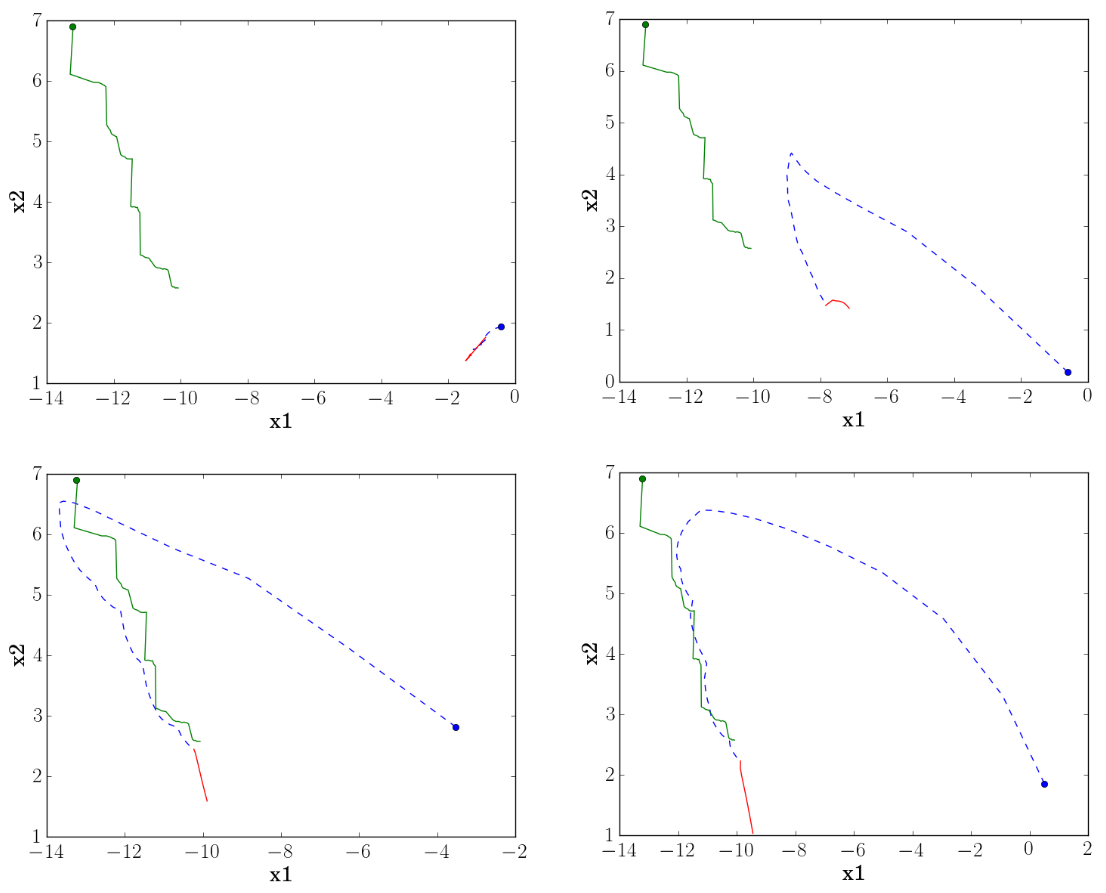
\includegraphics [trim=0 0 0 0, clip, angle=0, width=1.0\columnwidth,
	keepaspectratio]{figures/rnn_real_ped}
	\caption{Predictions on real pedestrian trajectory snippets. Colors are same as in~\cref{fig:rnn_hidden}. Search over the number of hidden units: $n_h=4$(top-left), $n_h=32$(top-right), $n_h=128$(bottom-left), $n_h=512$(bottom-right). The model with the highest complexity is able fit the pedestrian trajectories the best. The model is able to accurately predict the pedestrian's position one step ahead of time, given some observation time for convergence.}
	\label{fig:rnn_real_ped}
\end{figure}

\begin{table}[]
\centering
\begin{tabular}{ c| c| c| c| c}
& $n_h=4$ & $n_h=32$ &$n_h=128$ & $n_h=512$\\
\hline
$L_{e_c}$		&  50.3	& 21.8	& 4.6 & 1.8 	\\
$L_{test, e_c}$	& 18.46	& 4.43	& 0.81	& \textbf{0.11} 	\\     
\end{tabular}
\caption{Search over the number of hidden units $n_h$ results in the best performance with a model with 512 units. $L_{e_c}$ and $L_{test, e_c}$ is the average batch loss after convergence on the training and test data, respectively.}
\end{table}\label{tab:rnn_real_ped}

The model is able to predict the next pedestrian timestep with an error of $\sqrt{0.11}m$ on the test dataset.
As expected, our model was not able to predict pedestrian movement further than several timesteps. We expect better performance with more data and more extensive hyperparameter search.
However, pedestrians behave randomly, do not follow predestined rules, and different pedestrians behave differently.